\documentclass{beamer}
\usetheme{Warsaw}
%\usecolortheme{lily}

\title{Web People Search Task(WePS)}
\subtitle{Advaned NLP Project 2}
\author[Fan Kai , Wang Chen]{Fan Kai , Wang Chen \\ 10848194 10848263}
\institute{Peking University}
\date{2009.\alert{05.12}}

\begin{document}

\begin{frame}[label=titlepage]
    \titlepage
\end{frame}

\section{Introduction}
\begin{frame}{Major Tasks}
    \begin{itemize}
    \item Extract features from web pages.
    \item Calculate similarity between page pairs.
    \item Cluster similar web pages.
    \end{itemize}
\end{frame}

\begin{frame}{Thirdparty Tools and Environment}
    \begin{itemize}
    \item Jericho HTML Parser
    \item Stanford Named Entity Recognizer
    \item Natural Lauguage Toolkit(NLTK)
        \begin{itemize}
        \item Sentence Tokenizor
        \item Word Tokenizor
        \item Stop Words
        \item Portor Stemmer
        \end{itemize}
    \item Weka 3: Data Mining Software in Java
    \item Python 2.5
    \item Ubuntu 8.04
    \end{itemize}
\end{frame}
    
\section{Methodology}
\subsection{Feature Extraction}
\begin{frame}{Text Features}
    \begin{itemize}
    \item Full Text 
        Plain text extracted from web page.
    \item Text Summary 
        Sentences where names occurs.
    \item Metadata 
        Combination of title, snippet and url.
    \end{itemize}
\end{frame}

\begin{frame}{Named Entity Features}
    \begin{itemize}
    \item Person 
    \item Location
    \item Organization
    \end{itemize}
\end{frame}

\begin{frame}{Other Features}
    \begin{itemize}
    \item Link and URL
    \item Email Address
    \item Domain
    \item Number
    \item Telephone Number
    \item Year
    \end{itemize}
\end{frame}

\subsection{Similarity Calculation}
\begin{frame}{Similarity Calculation}
    \begin{itemize}
    \item Vector Space Model
        \begin{itemize}
        \item Calculate VSM similarity for each feature.
        \end{itemize}
    \item Machine Learning
        \begin{itemize}
        \item Learning Features: VSM similarity of each feature
        \item Learning Target: Probability two page indicate a single entity, used as similarity
        \item Methods
            \begin{itemize}
            \item Maximum Entropy
            \item Naive Bayes
            \item Decision Tree
            \end{itemize}
        \item Feature Selection
            \begin{itemize}
            \item All Features
            \item Text and Entity Features
            \end{itemize}
        \end{itemize}
    \end{itemize}
\end{frame}

\subsection{Clustering}
\begin{frame}{Clustering}
    \begin{itemize}
    \item Hierarchical Agglomerative Clustering
        \begin{itemize}
        \item fixed thresholds
        \item try different thresholds
        \item try different merge strategy
        \end{itemize}
    \item K-Means
        \begin{itemize}
        \item fixed cluster number
        \item try different cluster numbers
        \end{itemize}
    \end{itemize}
\end{frame}


\section{Results}
\subsection{Score}
\begin{frame}[plain]{Cluster Fulltext feature using K-Means(Test Set)}
\begin{figure}
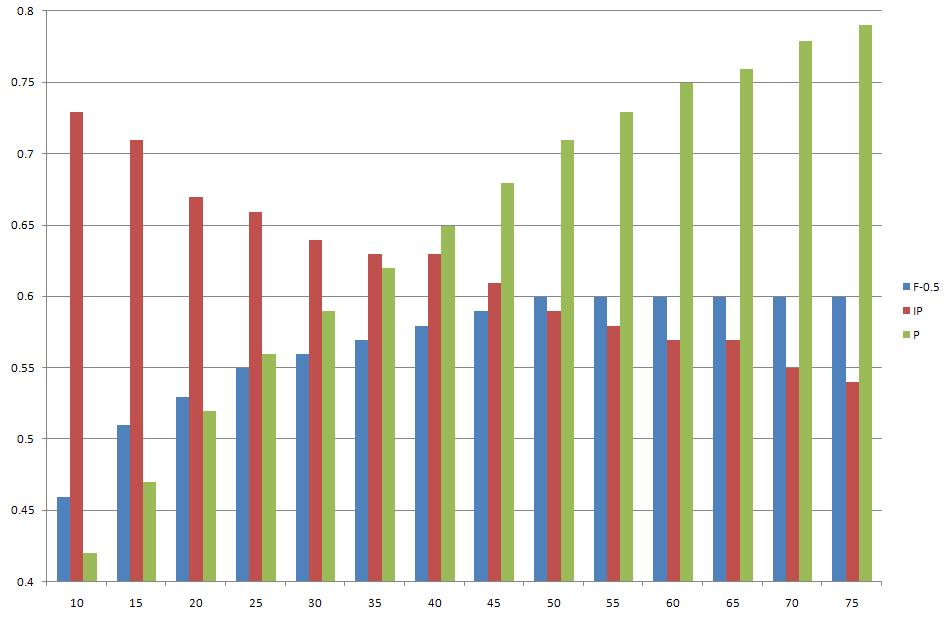
\includegraphics[width=100mm]{kmeans}
\end{figure}
\end{frame}

\begin{frame}[plain]{Cluster Fulltext feature using HAC(Test Set)}
\begin{figure}
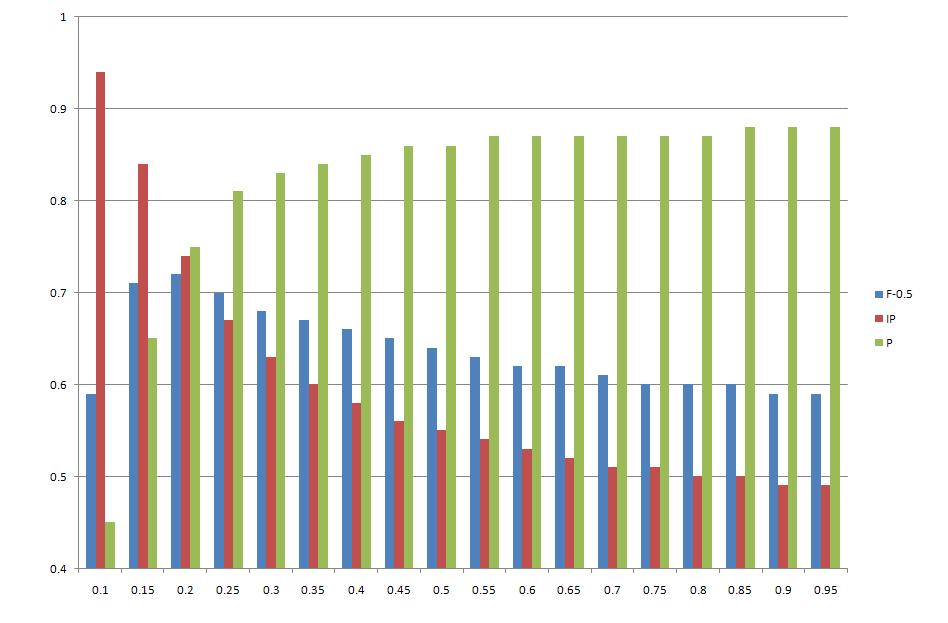
\includegraphics[width=100mm]{agglo}
\end{figure}
\end{frame}

\begin{frame}[plain]{FMeasure-0.5 with different HAC threshold(Test Set)}
\begin{figure}
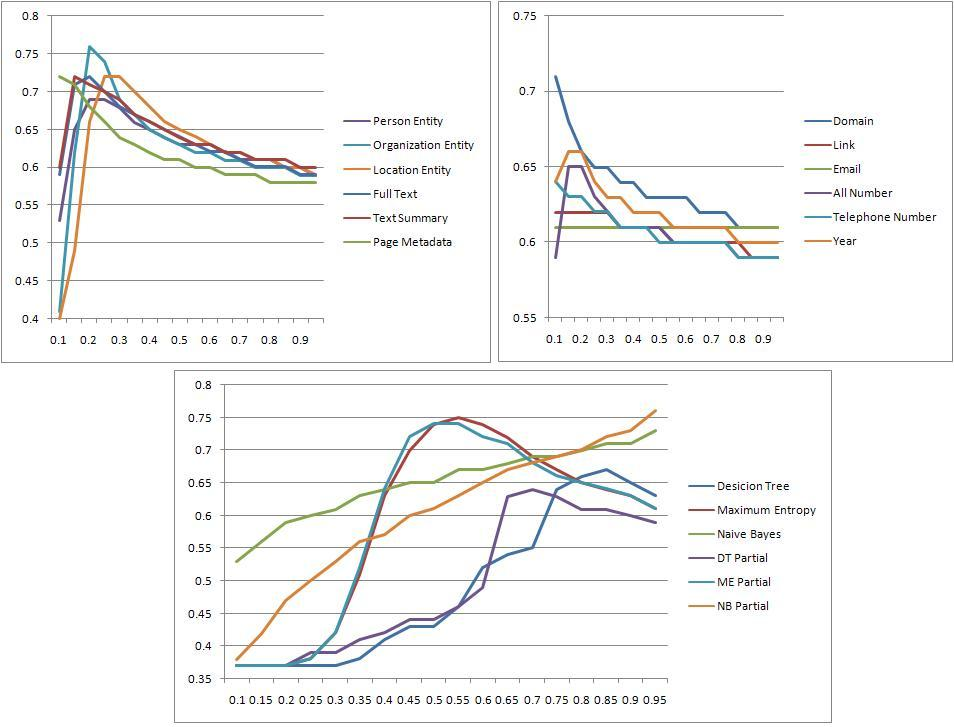
\includegraphics[width=100mm]{trend}
\end{figure}
\end{frame}

\begin{frame}[plain]{Best FMeasure-0.5(Test Set)}
\begin{figure}
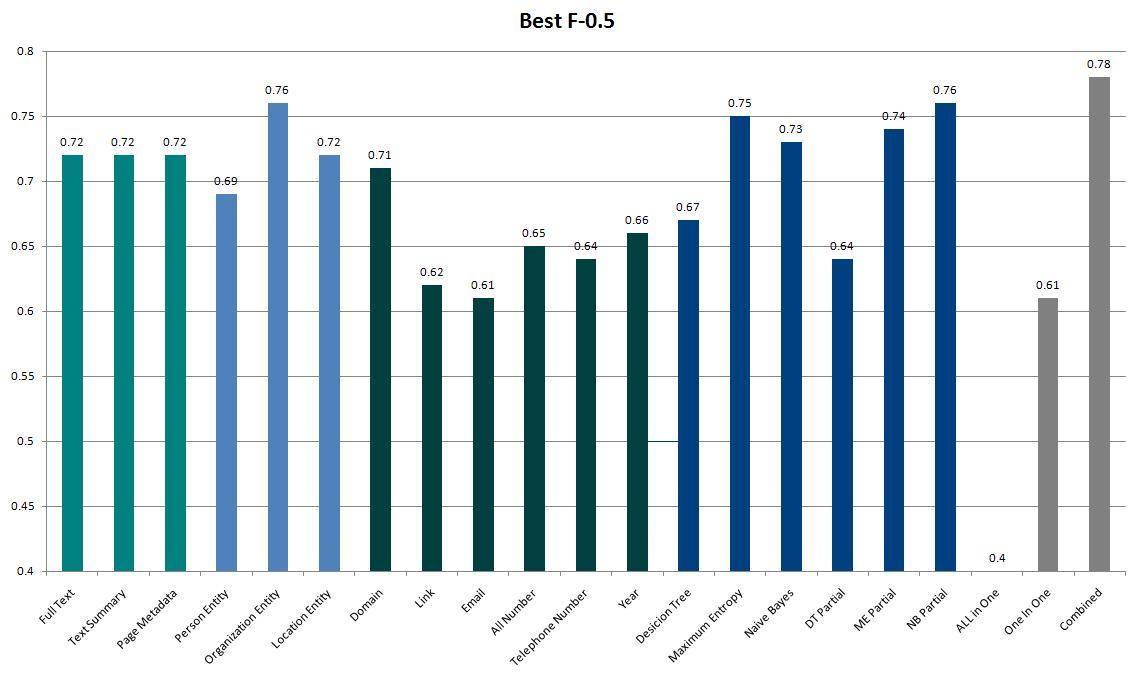
\includegraphics[width=100mm]{best}
\end{figure}
\end{frame}

\begin{frame}[plain]{Scores of Different Entities in Test Set(ME-0.55)}
\begin{figure}
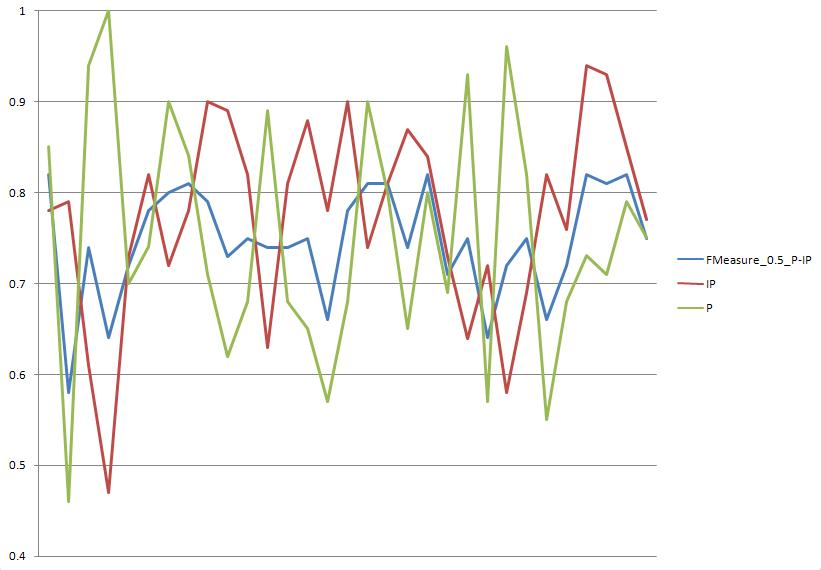
\includegraphics[width=100mm]{entity}
\end{figure}
\end{frame}

\begin{frame}[plain]{Comparison between Traing and Test Set}
\begin{figure}
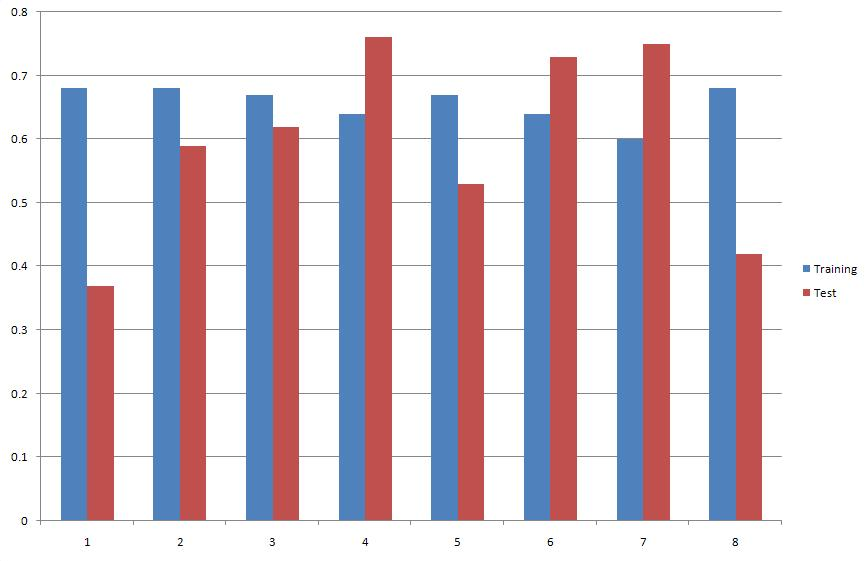
\includegraphics[width=100mm]{cmp}
\end{figure}
\end{frame}

\subsection{Other Issues}
\begin{frame}{Other Issues}
    \begin{itemize}
    \item Unknown character encodings.
    \item How to recognize discarded items?
        \begin{itemize}
        \item Couldn't find efficient judgement.
        \item Current condition: summary contains less than 5 words.
        \end{itemize}
    \end{itemize}
\end{frame}

\begin{frame}{How Discarded Items Matter(Test Set)}
\begin{figure}
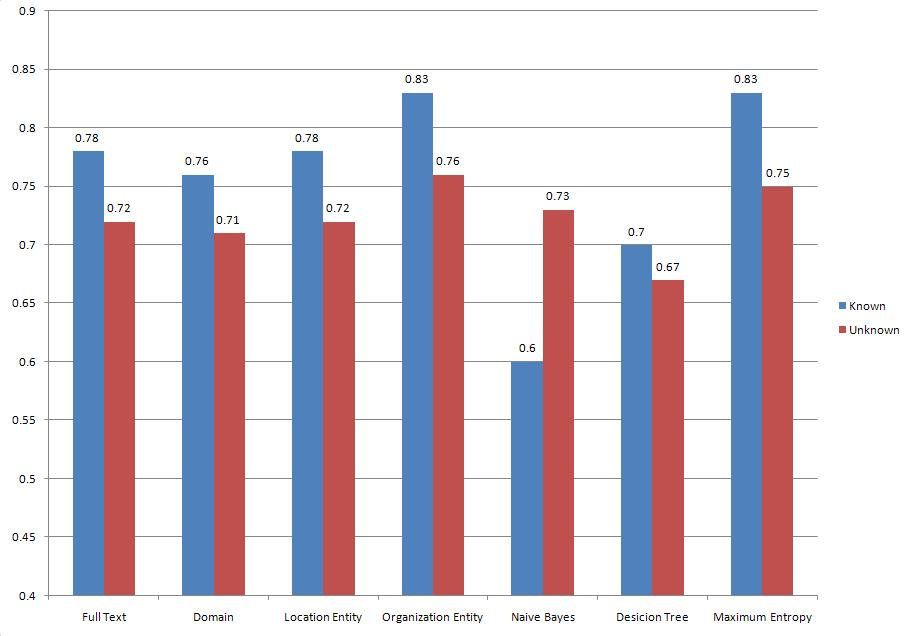
\includegraphics[width=100mm]{discard}
\end{figure}
\end{frame}

\subsection{Conclusion}
\begin{frame}{Best Scores}
\begin{itemize}
\item Using best result from traing set(fulltext-0.10):
%\vskip10pt
\begin{tabular}{|l|l|l|l|l|}
\hline
\textbf{Set} & \textbf{F-0.5} & \textbf{IP} & \textbf{P} \\
\hline
Training &  0.68 & 0.81 & 0.67 \\
\hline
Test&  0.59 & 0.94 & 0.45 \\
\hline
\end{tabular}
\item Discarded items unknown:
%\vskip10pt
\begin{tabular}{|l|l|l|l|l|}
\hline
\textbf{Similarity Type} & \textbf{Threshold} & \textbf{F-0.5} & \textbf{IP} & \textbf{P} \\
\hline
Organization Entity & 0.20 & 0.76 & 0.83 & 0.73 \\
\hline
Naive Bayes Partial & 0.95 & 0.76 & 0.84 & 0.71 \\
\hline
Maximum Entropy & 0.55 & 0.75 & 0.77 & 0.75 \\
\hline
\end{tabular}
%\vskip10pt
\item Discarded items known:
%\vskip10pt
\begin{tabular}{|l|l|l|l|l|}
\hline
\textbf{Similarity Type} & \textbf{Threshold} & \textbf{F-0.5} & \textbf{IP} & \textbf{P} \\
\hline
Organization Entity & 0.20 & 0.83 & 0.83 & 0.84 \\
\hline
Maximum Entropy & 0.95 & 0.83 & 0.82 & 0.86 \\
\hline
\end{tabular}
\end{itemize}
\end{frame}

\begin{frame}{Future Work}
    \begin{itemize}
    \item More features
    \item More sophisticated feature selection in ML
    \item Variable HAC threadhold or K-Means cluster number
    \end{itemize}
\end{frame}

\begin{frame}
\begin{center}\huge{Thanks!}\end{center}
\end{frame}

\end{document}


